\documentclass[border=10pt]{standalone}
\usepackage[svgnames]{xcolor}
\usepackage{amsmath}
\usepackage{pgfplots}
\pgfplotsset{compat=newest}
\usepackage[sfdefault]{FiraSans}
\usepackage{FiraMono}
\renewcommand*\familydefault{\sfdefault}
\begin{document}
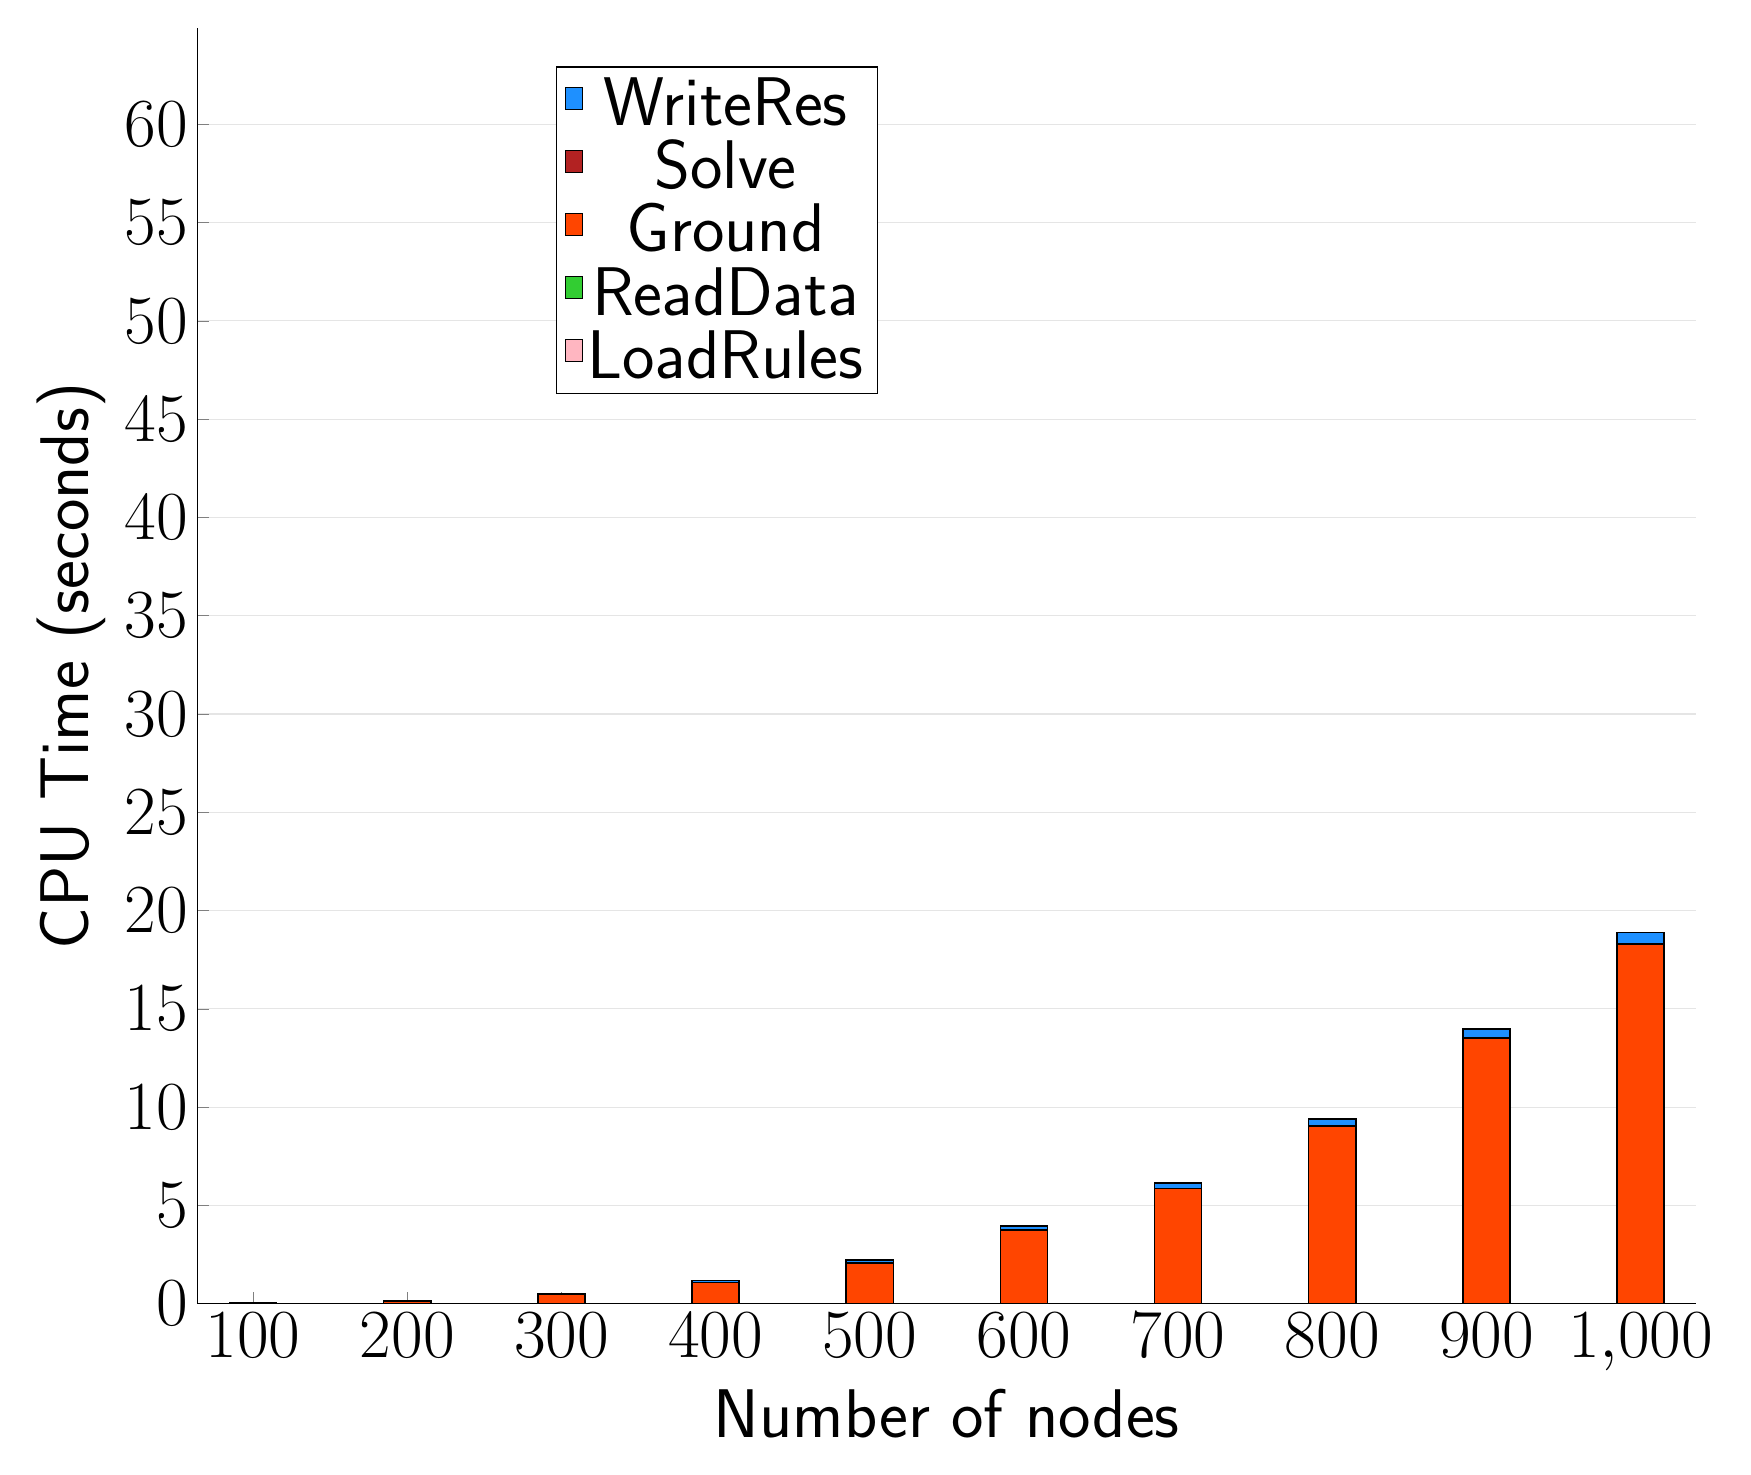
\begin{tikzpicture}
\begin{axis}[
   ybar stacked,
   width=1.7\textwidth,
   bar width=0.6cm,
   ymajorgrids, tick align=inside,
   major grid style={draw=gray!20},
   xtick=data,
   ymin=0, ymax=64.8926,
   axis x line*=bottom,
   axis y line*=left,
   enlarge x limits=0.04,
   legend style={
       at={(0.454, 0.97)},
       anchor=north east,
       legend columns=1,
       font=\Huge,
   },
   ylabel={CPU Time (seconds)},
   xlabel={Number of nodes},
   label style={font=\Huge},
   tick label style={font=\Huge},
]
\addlegendimage{fill=DodgerBlue, draw=black, line width=0.2pt}
\addlegendentry{WriteRes}
\addlegendimage{fill=FireBrick, draw=black, line width=0.2pt}
\addlegendentry{Solve}
\addlegendimage{fill=OrangeRed, draw=black, line width=0.2pt}
\addlegendentry{Ground}
\addlegendimage{fill=LimeGreen, draw=black, line width=0.2pt}
\addlegendentry{ReadData}
\addlegendimage{fill=LightPink, draw=black, line width=0.2pt}
\addlegendentry{LoadRules}
\addplot +[fill=LightPink, draw=black, line width=0.55pt] coordinates {
(100, 0.0)
(200, 0.0)
(300, 0.0)
(400, 0.0)
(500, 0.0)
(600, 0.0)
(700, 0.0)
(800, 0.0)
(900, 0.0)
(1000, 0.0)
};
\addplot +[fill=LimeGreen, draw=black, line width=0.55pt] coordinates {
(100, 0.0)
(200, 0.0)
(300, 0.0)
(400, 0.0)
(500, 0.0)
(600, 0.0)
(700, 0.0)
(800, 0.0)
(900, 0.0)
(1000, 0.0)
};
\addplot +[fill=OrangeRed, draw=black, line width=0.55pt] coordinates {
(100, 0.018000000000000016)
(200, 0.136)
(300, 0.458)
(400, 1.082)
(500, 2.06)
(600, 3.748)
(700, 5.854)
(800, 9.020000000000001)
(900, 13.488000000000003)
(1000, 18.286)
};
\addplot +[fill=FireBrick, draw=black, line width=0.55pt] coordinates {
(100, 0.0020000000000000018)
(200, 0.0020000000000000018)
(300, 0.0040000000000000036)
(400, 0.0040000000000000036)
(500, 0.0060000000000000496)
(600, 0.009999999999999875)
(700, 0.014000000000000058)
(800, 0.017999999999999617)
(900, 0.023999999999999844)
(1000, 0.029999999999999714)
};
\addplot +[fill=DodgerBlue, draw=black, line width=0.55pt] coordinates {
(100, -0.0020000000000000018)
(200, 0.02200000000000001)
(300, 0.04600000000000004)
(400, 0.09799999999999986)
(500, 0.14199999999999982)
(600, 0.20400000000000001)
(700, 0.2819999999999999)
(800, 0.36600000000000055)
(900, 0.4520000000000004)
(1000, 0.5780000000000003)
};
\end{axis}
\end{tikzpicture}

\end{document}
